\chapter{Conclusiones}

\section{Mejoras y ampliaciones}


\section{Modelo de negocio}

\begin{figure}
\begin{center}
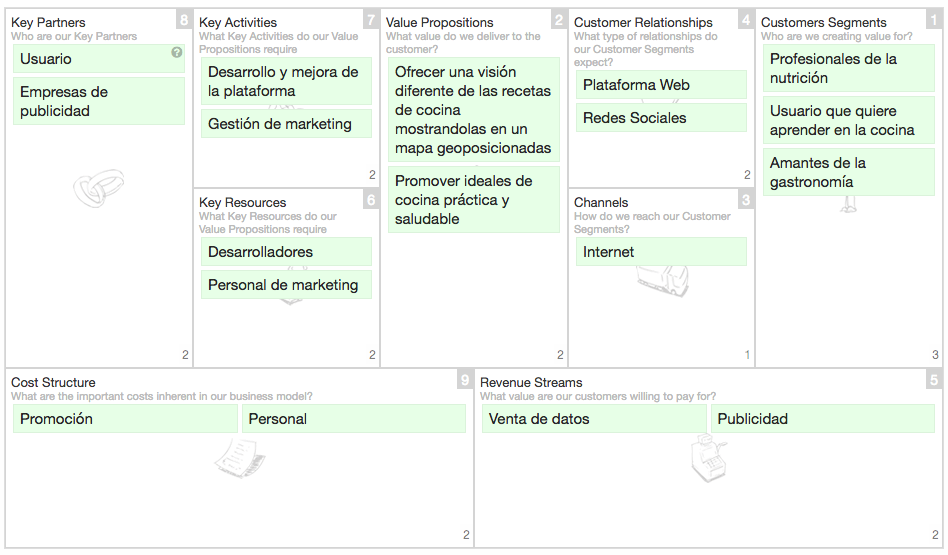
\includegraphics[width=1.0\textwidth]{imagenes/business-canvas.png}
\caption{Listado de elementos}
\label{business-canvas}
\end{center}
\end{figure}

Despues de desarrollar un producto mínimo viable de la aplicación de Njoycooking, se plantea la siguiente cuestión: ¿Es posible generar un modelo de negocio para la aplicación?

Mediante un business model canvas(figura \ref{business-canvas}) se describe de una forma simple en que consiste la idea de negocio.

\vspace{5 mm}

Al generar un modelo de negocio, el primer concepto que se tiene que valorar es: ¿Qué propuesta de valor ofrece la aplicación? es decir que elemento diferenciador puede ofrecer la aplicación frente otros existentes en el mercado. NjoyCooking es una aplicación gastronómica pero además de ofrecer un blog de cocina proporciona un visión diferente de los recetas de cocina, mostrando lo que cocina la gente según su zona geográfica mostrando las recetas geoposicionadas en un mapa y en tiempo real. Otra propuesta, es la de promover los hábitos de cocina práctica y saludable. 


\vspace{5 mm}

Otro concepto que se tiene que valorar es como relacionarse con el cliente. El principal punto de contacto con los clientes será la aplicación web, donde los usuarios podrán interactuar y conocer la propuesta de valor que ofrece. Otra forma de contactar será mediante las redes sociales, ya que son un medio de difusión muy importante para a dar a conocer la aplicación.

\vspace{5 mm}

¿De dónde se obtendrán los ingresos? Las principales fuentes de ingresos serán dos:

\begin{itemize}

\item \textbf{Publicidad}: se proporcionará a las empresas la posibilidad de anunciarse en el sitio web mediante banners.

\item \textbf{Venta de datos}: los datos recogidos en la aplicación se ofrecerán a cambio de un pago económico a las empresas interesadas. Pueden servir para empresas de publicidad para hacer estudios de mercado, sobre que productos son los usados según la región y poder usar esa información en su beneficio.

\end{itemize} 

\vspace{5 mm}

¿Cuales son las fuentes clave? ¿Es decir que personal se necesita para llevar a cabo la propuesta de valor? Para cumplir la propuesta de valor se necesitará la contratación de desarrolladores de software para desarrollar y mejorar la aplicación y especilistas en marketing para dar a conocer la aplicación y ofrecer un mejor uso y experiencia de ella.

\vspace{5 mm}

El usuario activo de la aplicación será el principal partner de la aplicación, ya que podrá promover la plataforma a sus conocidos y así abarcar un mayor número de usuarios. Las empresas de marketing y publicidad también se tienen en cuenta ya que pueden ayudar a llevar a cabo la propuesta de valor patrocinando el producto.


\vspace{5 mm}

Por último se debe tener en cuenta: ¿A qué público va enfocada la propuesta de valor? Pues NjoyCooking esta enfocada a un público bastante genérico como puede ser los amantes de la cocina. Aunque también se enfoca a usuarios primerizos en la cocina y profesionales de la nutrición.


